\documentclass{beamer}
\usefonttheme{professionalfonts}% Now beamer didn't modify the math fonts
\usepackage{geometry}
\usepackage[]{tcolorbox}
\usepackage{varwidth}   %% provides varwidth environment
\usepackage{empheq}
\usepackage{adjustbox}


\newcommand*{\cajados}[1]{\noindent\fbox{%
\parbox{\textwidth}{%
    #1
}%
}}
\newcommand{\caja}[1]{\begin{empheq}[box=\fbox]{alignat*=8}
    #1
\end{empheq}}

\newcommand*{\objetivodos}[2]{#1 x_{1} + #2 x_{2}}
\newcommand*{\objetivotres}[3]{#1 x_{1} + #2 x_{2} + #3x_{3}}
\newcommand*{\restdos}[3]{#1 x_{1} + #2 x_{2} \le #3}
\newcommand*{\irestdos}[3]{#1 x_{1}  #2 x_{2} = #3}
\newcommand*{\iresttres}[4]{#1 x_{1}  #2 x_{2} #3x_{3} = #4}

\newcommand*{\resttres}[4]{#1 x_{1} + #2 x_{2} + #3 x_{3} \le #4}
\newcommand*{\restuno}[2]{#1 x_{1} \le #2}
\newcommand{\posit}[1]{x_{#1} \ge 0}

\newcommand{\R}{\mathbb{R}}
% \usepackage{tikz-cd}
\beamertemplatenavigationsymbolsempty
\setbeamertemplate{footline}[page number]{}
\setbeamerfont{footline}{size=\footnotesize}
\usepackage{tcolorbox}
\usepackage{biblatex}
% \usepackage{tikzcd}
\usetheme{Copenhagen}
\usepackage{tikz}

\definecolor{asparagus}{rgb}{0.53, 0.66, 0.42}


\title[]{Clase tutorial 04: Programación entera.}
% \subtitle{Workshop de LOREL 2024.}
\date{28 de Agosto de 2024.}
\author[]{ Investigación operativa.
  }
\institute{Universidad de San Andrés}
% \titlegraphic{\hfill\includegraphics[height=1.5cm]{logo.pdf}}

\begin{document}
\maketitle

\begin{frame}{Objetivos de la clase de hoy.}
  La idea de la clase de hoy es ver los siguientes temas:
  \begin{itemize}
    \item Introducción a la Programación entera.
      \begin{itemize}
        \item Problema de asignación.
        \item Problema de inversión.
        \item Camino mínimo.
        \item Restricciones especiales.
      \end{itemize}
  \end{itemize}
\end{frame}


\begin{frame}[fragile]{Problema de asignación.}
  Una compañía decidió iniciar la producción de cuatro nuevos productos,
  usando tres fábricas que actualmente tienen capacidad ociosa. 


  Cada fábrica puede producir cualquiera de estos productos, excepto la fábrica 2 que no puede producir el producto 3.
  \pause

  Los productos requieren un esfuerzo productivo comparable por unidad; por lo tanto, la
  producción disponible se mide en unidades de cualquier producto que pueda
  fabricarse determinado día.

  Por cuestiones de logística la compañía no va a dividir la producción de un mismo producto en distintas fábricas.
  
  Nuestro objetivo es minimizar los costos de producción teniendo en cuenta estos requerimientos.
\end{frame}


\begin{frame}[fragile]{Problema de asignación: tablas}
  \begin{center}
    \begin{adjustbox}{width = 1.05 \textwidth}
        \begin{tabular}{|c |c | c | c| c| c|}
          \hline
          & \multicolumn{4}{|c|}{ Costo unitario (\$ por unidad)}  &  \\
          \hline
          Fábrica & Producto 1 & Producto 2 & Producto 3 & Producto 4 &  Capacidad por día \\
          \hline 
          1 & 41 & 27 & 28 & 24 & 55 \\
          2 & 40 & 29 & 0 & 23  & 75 \\
          3 & 37 & 30 & 27 & 21 & 45 \\
          \hline 
          Unidades por día & 20 & 30 & 30 & 40 & - \\
          \hline
        \end{tabular}
    \end{adjustbox}
  \end{center}
  Donde la última fila nos indica la cantidad de productos por día que debemos fabricar para alcanzar las ventas proyectadas.
\end{frame}


\begin{frame}[fragile]{Problema de asignación: tablas}
  
  Consideramos la tabla con la capacidad máxima de producción de cada producto por cada fábrica.


  \begin{center}
    \begin{adjustbox}{width = 1.05 \textwidth}
        \begin{tabular}{|c |c | c | c| c| c|}
          \hline
          & \multicolumn{3}{|c|}{ Costo total} & &  \\
          \hline
          Fábrica & Producto 1 & Producto 2 & Producto 3 & Producto 4 &  Capacidad por día \\
          \hline 
          1 & 41 $\cdot$ \alert{20} & 27 $\cdot$ \alert{30} & 28 $\cdot$ \alert{30} & 24 $\cdot$ \alert{40}& 55 \\
          2 & 40 $\cdot$ \alert{20} & 29 $\cdot$ \alert{30} & 0 $\cdot$ \alert{30}  & 23 $\cdot$ \alert{40} & 75 \\
          3 & 37 $\cdot$ \alert{20} & 30 $\cdot$ \alert{30} & 27 $\cdot$ \alert{30} & 21 $\cdot$ \alert{40} & 45 \\
          \hline 
          Unidades por día & 20 & 30 & 30 & 40 & - \\
          \hline
        \end{tabular}
    \end{adjustbox}
  \end{center}
\end{frame}

\begin{frame}[fragile]{Problema de asignación: tablas}
  \begin{center}
    \begin{adjustbox}{width = 1.05 \textwidth}
      \begin{tabular}{|c |c | c | c| c|}
        \hline
        & \multicolumn{3}{|c|}{ Costo total} &   \\
        \hline
        Fábrica & Producto 1 & Producto 2 & Producto 3 & Producto 4 \\
        \hline 
        1 & 820  & 810  & 840  & 960  \\
        2 & 800  & 870  & 0    & 920  \\
        3 & 740  & 900  & 810  & 840  \\
        \hline 
      \end{tabular}
    \end{adjustbox}
  \end{center}
\end{frame}

\begin{frame}[fragile]{Variables de decisión.}
  
  Consideramos las variables de decisión binarias 
  \[
    x_{ij} \in \{0,1\}, \ \ \ \forall i,j. \ \  1 \le i \le 3, \ 1 \le j \le 4
  \]
  donde: 
  \[
  x_{ij} = 
    \begin{cases}
      1 & \text{si asignamos el producto $j$ a la fábrica $i$  } \\
      0 & \text{si no} \\
    \end{cases}
  \]
\end{frame}

\begin{frame}[fragile]{Función objetivo.}
  Consideramos la matriz de costos 

  \[
    c_{ij} \in \Z, \  \ \  \forall i,j. \ \  1 \le i \le 3, \ 1 \le j \le 4
  \]

  donde $c_{ij}$ es el costo total de hacer el producto $j$ en la fábrica $i$.

  \pause 

  \bigskip

  De esta manera nuestra función objetivo resulta ser:

  \[
    Z  = \sum_{i=1}^{3} \sum_{j=1}^{4} c_{ij} x_{ij}
  \]

\end{frame}


\begin{frame}[fragile]{Restricciones.}
  \begin{itemize}
    \item Las fábricas $1$ y $2$ no pueden fabricar más de dos productos.
      \pause 
      \begin{align*}
        x_{11} + x_{12} + x_{13} + x_{14} & \le 2 \\
        x_{22} + x_{22} + x_{23} + x_{24} & \le 2 \\
      \end{align*}
      \pause 
      \item La fábrica $3$ no puede fabricar más de un producto.
      \[
        x_{31} + x_{32} + x_{33} + x_{34}  \le 1
      \]
  \end{itemize}
\end{frame}

\begin{frame}[fragile]{Restricciones.}
  \begin{itemize}
    \item Cada producto debe estar asignado a una sola fábrica.
    \pause 
      \begin{align*}
        x_{11} + x_{21} + x_{31} &= 1 \\
        x_{12} + x_{22} + x_{32} &= 1 \\
        x_{13} + x_{23} + x_{33} &= 1 \\
        x_{14} + x_{24} + x_{34} &= 1 \\
      \end{align*}
  \end{itemize}
\end{frame}

\begin{frame}[fragile]{Restricciones.}
  \begin{itemize}
    \item Cada fábrica tiene un límite de producción del cual no podemos excedernos.
    \pause 
      \begin{align*}
        20 \cdot x_{11}  + 30 \cdot x_{12}  + 30 \cdot x_{13}  + 40 \cdot x_{14}  & \le 55 \\
        20 \cdot x_{21}  + 30 \cdot x_{22}  + 30 \cdot x_{23}  + 40 \cdot x_{24}  & \le 75 \\
        20 \cdot x_{31}  + 30 \cdot x_{32}  + 30 \cdot x_{33}  + 40 \cdot x_{34}  & \le 45 \\
      \end{align*}
    \pause   
    \item La fábrica $2$ no puede producir el producto $3$.  
    \pause
      \[
        x_{23} = 0
      \]
  \end{itemize}
\end{frame}

\begin{frame}[fragile]{Solución.}
  Ya tenemos planteado el problema, pasamos a colab para resolver el problema.
  \href{https://colab.research.google.com/drive/1cPl8BasMrIC50dWZhoVIsz7EAYtN1h3w?usp=sharing}{Link a colab.}

  \pause 
  \bigskip 

  El valor óptimo resulta ser $3340$ y las variables de decisión (escritas de forma matricial) son: 
  \[
    x_{ij} = \matriz{0 & 1 & 0 & 0 \\ 1 & 0 & 0 & 1 \\ 0 & 0 & 1 & 0}
  \]

\end{frame}


\begin{frame}[fragile]{Problema de inversión.}
  Los integrantes de una mesa directiva están considerando 6 grandes inversiones. Cada una solo puede realizarse una vez. 
  Estas inversiones difieren en el valor presente del valor actual neto generado y además en el capital inicial requerido: 
  \bigskip 
  \begin{center}
    \begin{adjustbox}{width = 0.65 \textwidth}
      \begin{tabular}{|c |c | c | c| c| c | c|}
        \hline
        Inversión & 1 & 2 & 3 & 4 & 5 & 6 \\
        \hline 
        Ganancia & 15  & 12  & 16  & 18 & 9  & 11  \\
        Costo    & 38  & 33  & 39  & 45 & 23 & 27  \\
        \hline 
      \end{tabular}
    \end{adjustbox}
  \end{center}
\end{frame}

\begin{frame}[fragile]{Problema de inversión.}

  \begin{itemize}
    \item El capital total disponible es de 150.
    \item Las oportunidades de inversión 1 y 2 son mutuamente excluyentes, al igual que la 3 y 4. 
    \item La opción 4 no puede hacerse a menos que se lleve a cabo la 1 o la 2.
    \item No hay restricciones sobre las oportunidades 5 o 6.
  \end{itemize}

  \bigskip 
  \pause 

  El objetivo es seleccionar la combinación óptima de inversiones para maximizar la ganancia actualizada.
\end{frame}

\begin{frame}[fragile]{Variables de decisión y función objetivo.}
  
  Consideramos las variables de decisión binarias 
  \[
    x_{i} \in \{0,1\}, \ \ \ \forall i,. \ \  1 \le i \le 6
  \]
  donde: 
  \[
  x_{i} = 
    \begin{cases}
      1 & \text{si accedemos a la oportunidad de inversión $i$  } \\
      0 & \text{si no} \\
    \end{cases}
  \]

  \pause 

  Nuestra función objetivo está dada por 
  \[
    Z = \sum_{i=1}^{6} p_{i}x_{i} = 15x_{1} + 12x_{2} + 16x_{3} + 18x_{4} + 19x_{5} + 11x_{6}
  \]
  
  donde $p = (15,12,16,18,9,11)$ es el vector que tiene los valores de ganancia estimada.

\end{frame}

\begin{frame}[fragile]{Restricciones.}
  \begin{itemize}
    \item El capital total disponible es de 150.
    \pause 
      \[
        \sum_{i=1}^{6} c_{i}x_{i} =  38x_{1} + 33x_{2} + 39x_{3} + 45x_{4} + 23x_{5} + 27x_{6}
        \le 150
      \]
      donde $c = (38,33,39,45,23,27)$ es el vector de costos de las inversiones.
    
  \end{itemize}
\end{frame}

\begin{frame}[fragile]{Restricciones especiales.}
  \begin{itemize}
    \item Las oportunidades de inversión 1 y 2 son mutuamente excluyentes, al igual que la 3 y 4.
    \pause 
      \begin{align*}
        x_{1} + x_{2} &\le 1 \\
        x_{3} + x_{4} &\le 1 \\
      \end{align*}
    \pause   

    \item La opción 4 no puede hacerse a menos que se lleve a cabo la 1 o la 2.
    \pause 
    \[
      x_{4} \le x_{1} + x_{2}
    \]
  \end{itemize}
\end{frame}

\begin{frame}[fragile]{Solución.}
  Ya tenemos planteado el problema, pasamos a colab para resolver el problema.
  \href{https://colab.research.google.com/drive/1cPl8BasMrIC50dWZhoVIsz7EAYtN1h3w?usp=sharing}{Link a colab.}

  \pause 
  \bigskip 

  La ganancia óptima resulta ser $53$ y las variables de decisión
  \[
    x = (1,0,0,1,1,1).
  \]
\end{frame}

\begin{frame}[fragile]{Camino más corto.}
  Hallar el camino más corto que comienza en el nodo 0 y termina en el nodo 7.

  \bigskip
  
  \begin{center}
    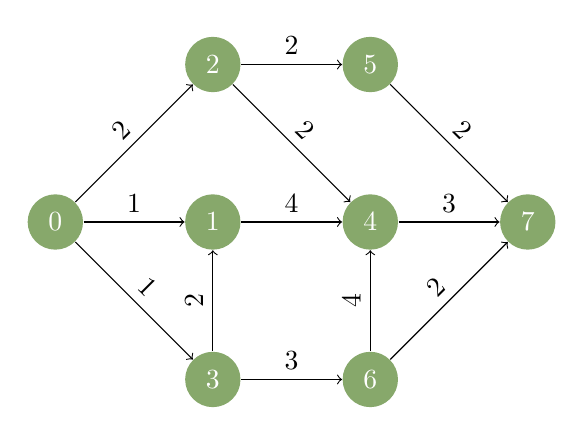
\begin{tikzpicture}
      \node[circle, fill=asparagus, minimum size=20pt, inner sep=0pt, text=white] (0) at (-6, 0) {0};
      \node[circle, fill=asparagus, minimum size=20pt, inner sep=0pt, text=white] (1) at (-4, 0) {1};
      \node[circle, fill=asparagus, minimum size=20pt, inner sep=0pt, text=white] (2) at (-4, 2) {2};
      \node[circle, fill=asparagus, minimum size=20pt, inner sep=0pt, text=white] (3) at (-4, -2) {3};
      \node[circle, fill=asparagus, minimum size=20pt, inner sep=0pt, text=white] (4) at (-2, 0) {4};
      \node[circle, fill=asparagus, minimum size=20pt, inner sep=0pt, text=white] (5) at (-2, 2) {5};
      \node[circle, fill=asparagus, minimum size=20pt, inner sep=0pt, text=white] (6) at (-2, -2) {6};
      \node[circle, fill=asparagus, minimum size=20pt, inner sep=0pt, text=white] (7) at (0, 0) {7};


      \foreach \i in {1, 6} {
          \foreach \j in {4} {
              \draw[->,bend right] (\i) -- (\j) node[midway, above, sloped] {4};
          }
      }
      \foreach \i in {0} {
          \foreach \j in {2} {
              \draw[->,bend right] (\i) -- (\j) node[midway, above, sloped] {2};
          }
      }
      \foreach \i in {0} {
          \foreach \j in {1,3} {
              \draw[->,bend right] (\i) -- (\j) node[midway, above, sloped] {1};
          }
      }
      \foreach \i in {2} {
          \foreach \j in {4,5} {
              \draw[->,bend right] (\i) -- (\j) node[midway, above, sloped] {2};
          }
      }
      \draw[->,bend right] (3) -- (1) node[midway, above, sloped] {2};
      \draw[->,bend right] (3) -- (6) node[midway, above, sloped] {3};
      \draw[->,bend right] (4) -- (7) node[midway, above, sloped] {3};
      \draw[->,bend right] (5) -- (7) node[midway, above, sloped] {2};
      \draw[->,bend right] (6) -- (7) node[midway, above, sloped] {2};
    \end{tikzpicture}
  \end{center}
\end{frame}

\begin{frame}[fragile]{Variables de decisión.}
  \begin{center}
    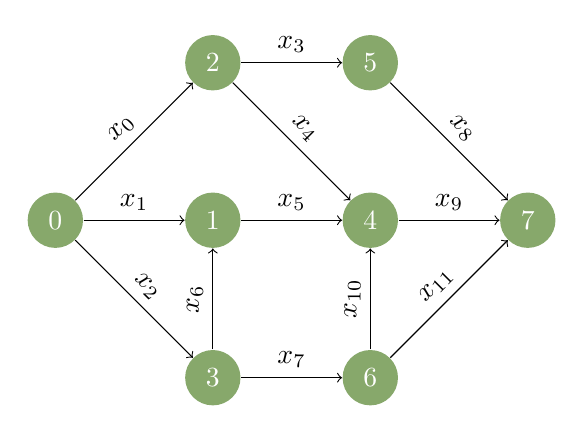
\begin{tikzpicture}
      \node[circle, fill=asparagus, minimum size=20pt, inner sep=0pt, text=white] (0) at (-6, 0) {0};
      \node[circle, fill=asparagus, minimum size=20pt, inner sep=0pt, text=white] (1) at (-4, 0) {1};
      \node[circle, fill=asparagus, minimum size=20pt, inner sep=0pt, text=white] (2) at (-4, 2) {2};
      \node[circle, fill=asparagus, minimum size=20pt, inner sep=0pt, text=white] (3) at (-4, -2) {3};
      \node[circle, fill=asparagus, minimum size=20pt, inner sep=0pt, text=white] (4) at (-2, 0) {4};
      \node[circle, fill=asparagus, minimum size=20pt, inner sep=0pt, text=white] (5) at (-2, 2) {5};
      \node[circle, fill=asparagus, minimum size=20pt, inner sep=0pt, text=white] (6) at (-2, -2) {6};
      \node[circle, fill=asparagus, minimum size=20pt, inner sep=0pt, text=white] (7) at (0, 0) {7};

      \draw[->,bend right] (0) -- (2) node[midway, above, sloped] {$x_{0}$};
      \draw[->,bend right] (0) -- (1) node[midway, above, sloped] {$x_{1}$};
      \draw[->,bend right] (0) -- (3) node[midway, above, sloped] {$x_{2}$};

      \draw[->,bend right] (2) -- (5) node[midway, above, sloped] {$x_{3}$};
      \draw[->,bend right] (2) -- (4) node[midway, above, sloped] {$x_{4}$};
      \draw[->,bend right] (1) -- (4) node[midway, above, sloped] {$x_{5}$};
      \draw[->,bend right] (3) -- (1) node[midway, above, sloped] {$x_{6}$};
      \draw[->,bend right] (3) -- (6) node[midway, above, sloped] {$x_{7}$};

      \draw[->,bend right] (5) -- (7) node[midway, above, sloped] {$x_{8}$};
      \draw[->,bend right] (4) -- (7) node[midway, above, sloped] {$x_{9}$};
      \draw[->,bend right] (6) -- (4) node[midway, above, sloped] {$x_{10}$};
      \draw[->,bend right] (6) -- (7) node[midway, above, sloped] {$x_{11}$};


    \end{tikzpicture}
  \end{center}
\end{frame}

\begin{frame}[fragile]{Variables de decisión.}
  Consideramos las variables de decisión binarias 
  \[
    x_{i} \in \{0,1\}, \ \ \ \forall i. \ \  1 \le i \le 11
  \]
  donde: 
  \[
  x_{i} = 
    \begin{cases}
      1 & \text{si usamos la arista $i$ en el camino } \\
      0 & \text{si no} \\
    \end{cases}
  \]
\end{frame}

\begin{frame}[fragile]{Función objetivo.}
  Sea $d = (2,1,1,2,2,4,2,3,2,3,4,2)$ el vector de las distancias de las aristas luego queremos minimizar la siguiente función 

  \[
    Z = \sum_{i=1}^{11} d_{i}x_{i}
  \]
  
\end{frame}

\begin{frame}[fragile]{Restricciones.}
  Tenemos las restricciones de flujo. 
  Por cada nodo conseguimos lo siguiente:
  \begin{itemize}
    \item Nodo 0.
      \[
        x_{0} + x_{1} + x_{2} = 1
      \]

    \item Nodo 1.
      \[
        x_{1} + x_{6} = x_{5}
      \]
    \item Etc.
  \end{itemize}
  \bigskip 
  \alert{Terminar el planteo y resolverlo en Python.}
  
\end{frame}

\begin{frame}[fragile]{Tarea.}
  \tcajita{Problema}{Una empresa tiene 2 turnos productivos. Sin importar la cantidad producida, el único costo es el de puesta en marcha del turno.
  Cuesta \$8000 ejecutar el turno diurno y \$4.500 el turno nocturno.
  La demanda para los próximos días es la siguiente:
    \begin{itemize}
      \item Día 1: 2.000; 
      \item Noche 1: 3.000;
      \item Día 2: 2.000;
      \item Noche 2: 3.000.
    \end{itemize}
  Cuesta \$1 por unidad stockear.
  Determinar el programa de producción óptimo que minimice el costo total cumpliendo la demanda.}
\end{frame}

\end{document}
